\chapterimage{MathCover.png}
\chapter{Water Math - Week 5}



\begin{table}[H]
\begin{tabular}{| m{1cm} | m{1cm} | m{12cm} |}
\hline
\multicolumn{3}{|l|}{\textbf{Expected   Range of Knowledge for Math}}                                                                      \\ \hline
\multicolumn{3}{|l|}{\textit{Water   Distribution System Operator License Exams}}                                                          \\ \hline
\multicolumn{1}{l|}{} & \multicolumn{1}{l|}{D1-D5} & Ability to calculate   flow rates for a storage facility                     \\ \cline{2-3} 
\multicolumn{1}{l|}{} & \multicolumn{1}{l|}{D1-D5} & Ability to calculate   the volume of a storage facility                      \\ \cline{2-3} 
\multicolumn{1}{l|}{} & \multicolumn{1}{l|}{D1-D5} & Knowledge of unit   conversions                                              \\ \cline{2-3} 
\multicolumn{1}{l|}{} & \multicolumn{1}{l|}{D1-D5} & Ability to calculate   flow rates                                            \\ \cline{2-3} 
\multicolumn{1}{l|}{} & \multicolumn{1}{l|}{D1-D5} & Ability to calculate   pipe volumes                                          \\ \cline{2-3} 
\multicolumn{1}{l|}{} & \multicolumn{1}{l|}{D1-D5} & Ability to calculate   the area of a pipe cross-section                      \\ \cline{2-3}
\multicolumn{1}{l|}{} & \multicolumn{1}{l|}{D1-D5} & Ability to calculate   the volume of a trench                                \\ \cline{2-3}  
\multicolumn{1}{l|}{} & \multicolumn{1}{l|}{D1-D5} & Ability to calculate   the surface area of a valve face                      \\ \cline{2-3} 
\multicolumn{1}{l|}{} & \multicolumn{1}{l|}{D1-D5} & Ability to calculate   the volume of a cylinder, rectangle, and square       \\ \cline{2-3} 
\multicolumn{1}{l|}{} & \multicolumn{1}{l|}{D1-D5} & Ability to calculate   the volume of a pipe                                  \\ \cline{2-3} 
\multicolumn{1}{l|}{} & \multicolumn{1}{l|}{D1-D5} & Ability to calculate   the volume of a well, storage reservoir, pipe, trench \\ \cline{2-3} 
\multicolumn{1}{l|}{} & \multicolumn{1}{l|}{D1-D5} & Ability to calculate   the well draw down                                    \\ \cline{2-3} 
\multicolumn{1}{l|}{} & \multicolumn{1}{l|}{D1-D5} & Ability to calculate   total force on a valve                                \\ \cline{2-3} 
\multicolumn{1}{l|}{} & \multicolumn{1}{l|}{D1-D5} & Ability to convert   pressure to feet of head                                \\ \cline{2-3} 
\multicolumn{1}{l|}{} & \multicolumn{1}{l|}{D1-D5} & Ability to convert   units of volume, area, and time                         \\ \cline{2-3} 
\multicolumn{1}{l|}{} & \multicolumn{1}{l|}{D1-D5} & Ability to convert   units of volume, area, pressure, and time               \\ \cline{2-3} 
\multicolumn{1}{l|}{} & \multicolumn{1}{l|}{D1-D5} & Ability to convert   units of volume, pressure and area                      \\ \cline{2-3} 
\multicolumn{1}{l|}{} & \multicolumn{1}{l|}{D1-D5} & Ability to convert   water units                                             \\ \cline{2-3} 
\multicolumn{1}{l|}{} & \multicolumn{1}{l|}{D2-D5} & Ability to calculate   pipe capacity                                         \\ \cline{2-3} 
\multicolumn{1}{l|}{} & \multicolumn{1}{l|}{D2-D5} & Ability to calculate   the velocity of water                                 \\ \cline{2-3} 
\multicolumn{1}{l|}{} & \multicolumn{1}{l|}{D2-D5} & Ability to calculate   thrust block size                                     \\ \cline{2-3} 
\multicolumn{1}{l|}{} & \multicolumn{1}{l|}{D2-D5} & Ability to convert a   pressure reading to depth of water                    \\ \cline{2-3} 
\multicolumn{1}{l|}{} & \multicolumn{1}{l|}{D2-D5} & Ability to convert a   scale to actual distance                              \\ \cline{2-3} 
\end{tabular}
\end{table}
\newpage






\begin{table}[H]
\begin{tabular}{| m{1cm} | m{1cm} | m{12cm} |}
\hline
\multicolumn{3}{|l|}{\textbf{Expected   Range of Knowledge for Math}}                                                                      \\ \hline
\multicolumn{3}{|l|}{\textit{Water   Distribution System Operator License Exams (Continued)}}                                                          \\ \hline
\multicolumn{1}{l|}{} & \multicolumn{1}{l|}{D3-D5} & Ability to calculate   brake-horsepower                                      \\ \cline{2-3} 
\multicolumn{1}{l|}{} & \multicolumn{1}{l|}{D3-D5} & Ability to calculate   pump efficiency                                       \\ \cline{2-3} 
\multicolumn{1}{l|}{} & \multicolumn{1}{l|}{D3-D5} & Ability to calculate   specific yield of a well                              \\ \cline{2-3} 
\multicolumn{1}{l|}{} & \multicolumn{1}{l|}{D3-D5} & Ability to calculate   the cost of water production                          \\ \cline{2-3} 
\multicolumn{1}{l|}{} & \multicolumn{1}{l|}{D4-D5} & Ability to calculate a water loss rate                                       \\ \cline{2-3} 
\multicolumn{1}{l|}{} & \multicolumn{1}{l|}{D4-D5} & Ability to calculate the cost of pumping   water                             \\ \cline{2-3} 
\multicolumn{1}{l|}{} & \multicolumn{1}{l|}{D4-D5} & Ability to calculate the hydraulic gradient                                  \\ \cline{2-3} 
\multicolumn{1}{l|}{} & \multicolumn{1}{l|}{D4-D5} & Ability to calculate water production costs                                  \\ \hline
\multicolumn{3}{|l|}{Water   Treatment Operator License Exams}                                                                    \\ \hline
\multicolumn{1}{l|}{} & \multicolumn{1}{l|}{T1-T4} & Ability to calculate   flow rates and water velocity                         \\ \cline{2-3} 
\multicolumn{1}{l|}{} & \multicolumn{1}{l|}{T1-T4} & Ability to calculate   the volume of water in a storage facility             \\ \cline{2-3} 
\multicolumn{1}{l|}{} & \multicolumn{1}{l|}{T1-T4} & Ability to calculate   well head pressure                                    \\ \cline{2-3} 
\multicolumn{1}{l|}{} & \multicolumn{1}{l|}{T1-T4} & Ability to convert   common water units (e.g. gallons per minute to MGD)     \\ \cline{2-3} 
\multicolumn{1}{l|}{} & \multicolumn{1}{l|}{T1-T4} & Ability to convert   head pressure to water elevation                        \\ \cline{2-3} 
\multicolumn{1}{l|}{} & \multicolumn{1}{l|}{T1-T4} & Ability to convert   units of length, volume, flow and pressure              \\ \cline{2-3} 
\multicolumn{1}{l|}{} & \multicolumn{1}{l|}{T1-T4} & Ability to determine   water level in a storage tank, reservoir, or well     \\ \cline{2-3} 
\multicolumn{1}{l|}{} & \multicolumn{1}{l|}{T1-T4} & Ability to calculate   a chemical dosage                                     \\ \cline{2-3} 
\multicolumn{1}{l|}{} & \multicolumn{1}{l|}{T1-T4} & Ability to calculate   a chemical solution concentration                     \\ \cline{2-3} 
\multicolumn{1}{l|}{} & \multicolumn{1}{l|}{T1-T4} & Ability to calculate   chlorine demand and chlorine residual                 \\ \cline{2-3} 
\multicolumn{1}{l|}{} & \multicolumn{1}{l|}{T1-T4} & Ability to convert   common water units, (gallons per minute to MGD, etc...) \\ \cline{2-3} 
\multicolumn{1}{l|}{} & \multicolumn{1}{l|}{T1-T4} & Ability to determine   water level in a storage tank, reservoir or well      \\ \cline{2-3} 
\multicolumn{1}{l|}{} & \multicolumn{1}{l|}{T3-T4} & Ability to perform   blending calculations                                   \\ \cline{2-3} 
\multicolumn{1}{l|}{} & \multicolumn{1}{l|}{T3-T4} & Ability to calculate   a dilution factor                                     \\ \cline{2-3} 
\multicolumn{1}{l|}{} & \multicolumn{1}{l|}{T3-T4} & Ability to mix   chemicals and prepare reagents                              \\ \cline{2-3} 
\multicolumn{1}{l|}{} & \multicolumn{1}{l|}{T3-T4} & Ability to perform   dilutions                                               \\ \cline{2-3} 
\multicolumn{1}{l|}{} & \multicolumn{1}{l|}{T3-T4} & Ability to calculate   a coagulant dose from a jar test                      \\ \cline{2-3} 
\multicolumn{1}{l|}{} & \multicolumn{1}{l|}{T3-T4} & Ability to calculate   a filter-aid dosage                                   \\ \cline{2-3} 
\multicolumn{1}{l|}{} & \multicolumn{1}{l|}{T3-T4} & Ability to calculate   a filtration rate                                     \\ \cline{2-3} 
\multicolumn{1}{l|}{} & \multicolumn{1}{l|}{T3-T4} & Ability to calculate   filter loading rate                                   \\ \cline{2-3} 
\multicolumn{1}{l|}{} & \multicolumn{1}{l|}{T3-T4} & Ability to calculate   percent or log removal of contaminants from water     \\ \cline{2-3} 
\multicolumn{1}{l|}{} & \multicolumn{1}{l|}{T3-T4} & Ability to calculate   the cost of water treatment operations                \\ \cline{2-3} 
\end{tabular}
\end{table}
\newpage


\section{Force, Pressure and Head} \index{Force, Pressure and Head}

\textbf{Force:}  In the English system force and weight are often used in the same way. The weight of the cubic foot of water is $62.4$ pounds. The force exerted on the bottom of the one foot cube is $62.4$ pounds. If we have two cubes stacked on top of one another, the force on the bottom will be $124.8$ pounds.

\textbf{Pressure:} Pressure is a force per unit of area, pounds per square inch or pounds per square foot are common expressions of pressure. 

\textbf{Head:}  Pressure is directly related to the height of a column of fluid. This height is called head or feet of head. Pressure and feet of head head are directly related - \emph{for every one foot of head there is a pressure of $0.433$ psi.}

\vspace{0.2cm}
Thus, $\dfrac{0.433 \enspace psi}{ft \enspace (water \enspace column)}$ or conversely $\dfrac{1 \enspace ft \enspace (water \enspace column)}{2.31 \enspace psi}$\\
\texthl{Note:  This pressure/head will include the height the water pumped and also the head associated with friction losses - energy loss because of the water moving through the pipe and fittings.}\\

\begin{figure}[h]
\begin{tikzpicture}
\path[help lines,step=.2] (0,0) grid (16,6);
\path[help lines,line width=.6pt,step=1] (0,0) grid (16,6);
%\foreach \x in {0,1,2,3,4,5,6,7,8,9,10,11,12,13,14,15,16}
%\node[anchor=north] at (\x,0) {\x};
%\foreach \y in {0,1,2,3,4,5,6}
%\node[anchor=east] at (0,\y) {\y};
\pgfmathsetmacro{\cubex}{3}
\pgfmathsetmacro{\cubey}{3}
\pgfmathsetmacro{\cubez}{3}
\draw(13.5,5,3) -- ++(-\cubex,0,0) -- ++(0,-\cubey,0) -- ++(\cubex,0,0) -- cycle;
\draw(13.5,5,3) -- ++(0,0,-\cubez) -- ++(0,-\cubey,0) -- ++(0,0,\cubez) -- cycle;
\draw(13.5,5,3) -- ++(-\cubex,0,0) -- ++(0,0,-\cubez) -- ++(\cubex,0,0) -- cycle;
\draw (8.7,2.5) node[text width=3cm,align=center]
  {\scriptsize{12"}};
\draw (14.1,3.4) node[text width=3cm,align=center]
  {\scriptsize{12"}};
  \draw (10.9,0.5)node[text width=3cm,align=center]
  {\scriptsize{12"}};
    \draw (2.8,4.8)node[text width=3.8cm,align=left]
  {\small{$Pressure=\dfrac{Force}{Area}$}};
      \draw (2.8,3.1)node[text width=3.8cm,align=left]
  {\small{Pressure exerted by}};
        \draw (2.8,2.8)node[text width=3.8cm,align=left]
  {\small{a 1ft column of water}};
        \draw (5.3,2.9)node[text width=3cm,align=center]
  {\small{$=\dfrac{62.4 \enspace lb}{12 in \enspace x \enspace 12 in}$}};
          \draw (7.3,2.9)node[text width=3cm,align=center]
  {\small{$=0.43 \enspace psi$}};
         \draw (3.45,1.2)node[text width=5cm,align=left]
  {\small{As 1$ft^3$ of water weighs 62.4 lbs}};
\end{tikzpicture}
\end{figure}


The pressure at the bottom of a container is affected only by the height of water in the container and not by the shape or the volume of the container. In the drawing below there are four containers all of different shapes and sizes. The pressure at the bottom of each is the same.

\begin{center}
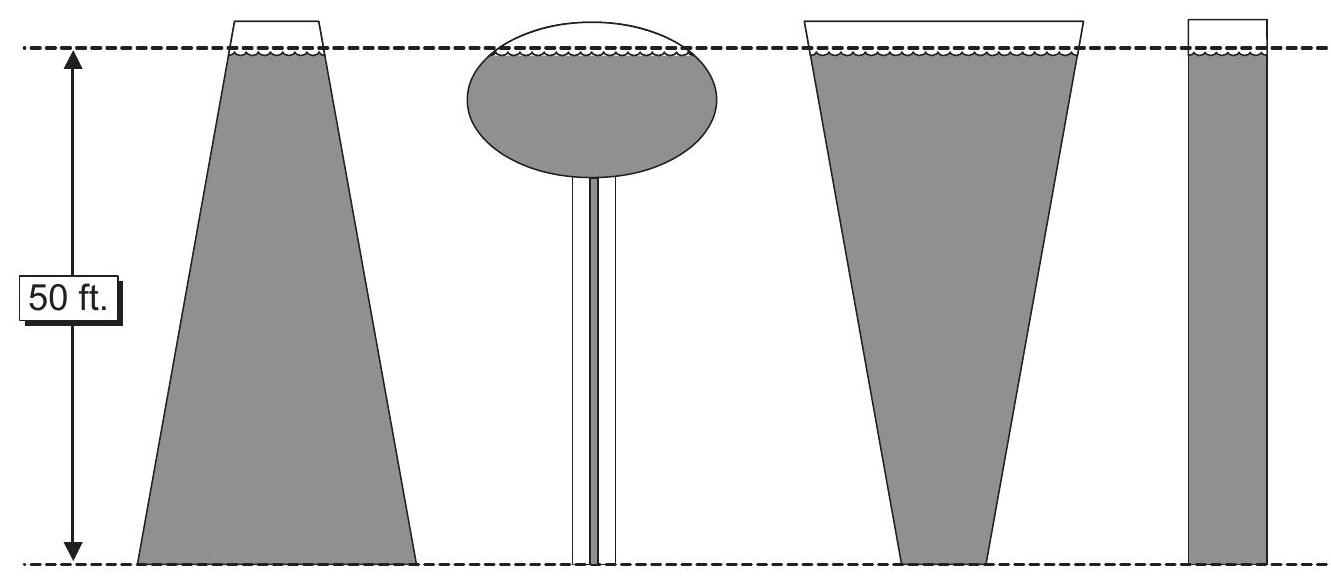
\includegraphics[scale=0.2]{2022_11_03_65aa625ded296bdfd01fg-17}
\end{center}
The pressure exerted at the bottom of a tank is relative only to the head on the tank and not the volume of water in the tank. For example, below are two tanks each containing 5000 gallons. The pressure at the bottom of each is 22 psi. If half of the water were drained from the tanks the pressure at the bottom of the elevated tank would be $17.3$ psi while the pressure at the bottom of the standpipe would be 11 psi.\\

\begin{center}
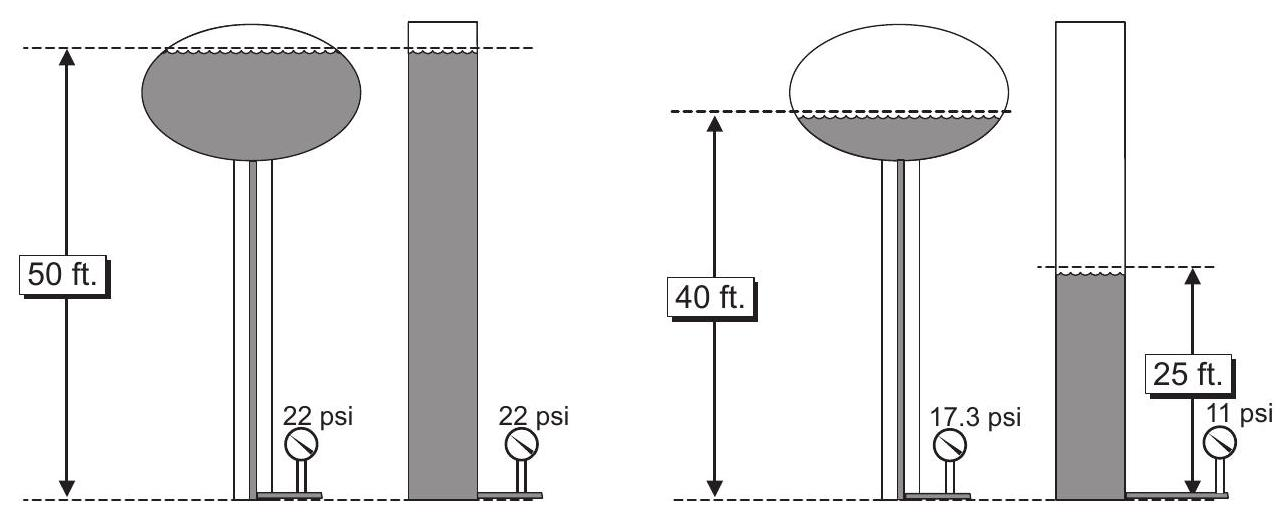
\includegraphics[scale=0.25]{2022_11_03_65aa625ded296bdfd01fg-18}
\end{center}


\begin{itemize}
\item A reservoir is 40 feet tall. Find the pressure at the bottom of the reservoir.

$40 \mathrm{ft} \times 0.433 \mathrm{psi} / \mathrm{ft}=17.3 \mathrm{psi}$

\vspace{0.4cm}

\item Find the height of water in a tank if the pressure at the bottom of the tank is 12 psi.

$12 \mathrm{psi} \div 0.433 \mathrm{psi} / \mathrm{ft}=27.7 \mathrm{ft}$

\vspace{0.4cm}

\item If a pump discharge pressure gauge read 10 psi, the height of the water corresponding to this pressure would be:
$$10 \enspace psi \times \dfrac{2.31 \enspace ft}{psi}=23.1 \enspace ft$$\\
\vspace{0.4cm}
\end{itemize}

% \begin{tcolorbox}[breakable, enhanced,
% colframe=blue!25,
% colback=blue!10,
% coltitle=blue!20!black,  
% title= Practice Problems]

% \begin{enumerate}
% \item Convert 45 psi to feet of head

% \item If the pressure at a water main is 50 psi, what would the static pressure (psi) be at a faucet on the top floor of a four story building? (Assuming 10 ft. per story)

% \item A water tower has water pressure of 98 psi at its base. What would be. the pressure at a hydrant three blocks away if there is a 65-foot head loss in the pipe?\\

% \end{enumerate}

% \end{tcolorbox}






\section{Pumping Calculations}\index{Pumping Calculations}
\begin{itemize}
\item Pump is a machine used for moving water (and other fluids) through a piping system and raise the pressure of the water.
\item Pumping is accomplished by transforming the input energy - typically from an electric motor or from other sources such as high-pressure air.
\item The pump calculations in this section are for electrically driven rotodynamic pumps.
\item To move water, a pump will need to overcome resistance due its density, gravitational force and friction.
\item This resistance is dependent on:
\begin{itemize}
\item Height the water needs to be raised.  This height of the fluid in a container is referred to as head. 
\item Quantity of water involved
\end{itemize}
\end{itemize}

\subsection{Glossary of Pump Calculations Terms}\index{Glossary of Pump Calculations Terms}

\textbf{Static Pressure: } Static implies a non-moving condition.  The pressure measured when there is no water moving in a line or the pump is not running is called static $^{32}$ pressure. This is the pressure represented by the gauges on the tanks in the discussion above.

\textbf{Dynamic Pressure: } When water is allowed to run through a pipe and the pressure (called pressure head) measured at various points along the way we find that the pressure decreases the further we are from the sources.
\begin{center}
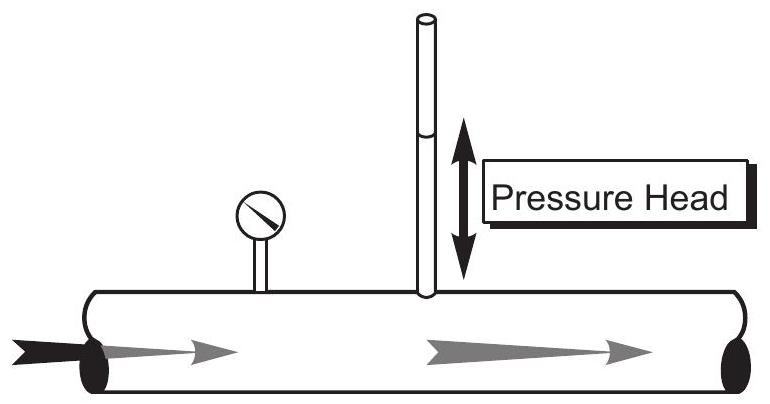
\includegraphics[scale={0.2}]{2022_11_03_65aa625ded296bdfd01fg-18(1)}
\end{center}
\textbf{Headloss: }  The reason for this reduction in pressure is a phenomenon called headloss. Headloss is the loss of energy (pressure) due to friction. The energy is lost as heat.

If the headloss in a certain pipe is 25 feet, it means the amount of energy required to overcome the friction in the pipe is equivalent to the amount of energy that would be required to lift this amount of water straight in the air 25 feet.

In a pipe, the factors that contribute to headloss include the following:

\begin{itemize}
  \item Roughness of pipe - If the roughness of a pipe were doubled the headloss would double.

  \item Length of pipe - If the length of the pipe were doubled the headloss would double.

  \item Diameter of pipe - If the diameter of a pipe were doubled the headloss would be cut in half

  \item Velocity of water - If the velocity of the water in a pipe were doubled the headloss would be increased by about four times. It should be apparent that velocity, more than any other single factor, affects headloss. To double the velocity we would have to double the flow in the line.
  
  \item Pumping System Components and Fittings - Each type of fitting has a specific headloss depending upon the velocity of water through the fitting. For instance the headloss though a check valve is two and one quarter times greater than through a ninety degree elbow and ten times greater than the headloss through an open gate valve.

\end{itemize}

\textbf{Static Head: }  Static head is the distance between the suction and discharge water levels when the pump is shut off. 

\textbf{Suction Lift: } Suction lift is the distance between the suction water level and the center of the pump impeller. This term is only used when the pump is in a suction lift condition. A pump is said to be in a suction lift condition any time the eye (center) of the impeller is above the water being pumped.

\textbf{Velocity Head: } The amount of energy required to bring a fluid from standstill to its velocity. For a given quantity of flow, the velocity head will vary indirectly with the pipe diameter.

\textbf{Total Dynamic Head (TDH):}  The total energy needed to move water from the center line of a pump (eye of the first impeller of a lineshaft turbine) to some given elevation or to develop some given pressure. This includes the static head, velocity head and the headloss due to friction. 

\textbf{Horsepower: } Horsepower is a measurement of the amount of energy required to do work. Motors are rated in horsepower. The horsepower of an electric motor is called brake horsepower. The horsepower requirements of a pump are dependent on the flow and the total dynamic head.  33,000 foot pounds per minute of work is 1 horsepower.

\textbf{Suction Head: } Suction head is the distance between the suction water level and the center of the pump impeller when the pump is in a suction head condition. A pump is said to be in a suction head condition any time the eye (center) of the impeller is below the water level being pumped.

\textbf{Velocity Head: } Velocity head is the amount of energy required by the pump and motor to overcome inertia and bring the water up to speed. Velocity head is often shown mathematically as $\mathrm{V}^{2} / 2 \mathrm{~g}$. ( $\mathrm{g}$ is the acceleration due to gravity $-32.2 \mathrm{ft} / \mathrm{sec}^{2}$ ).
\begin{center}
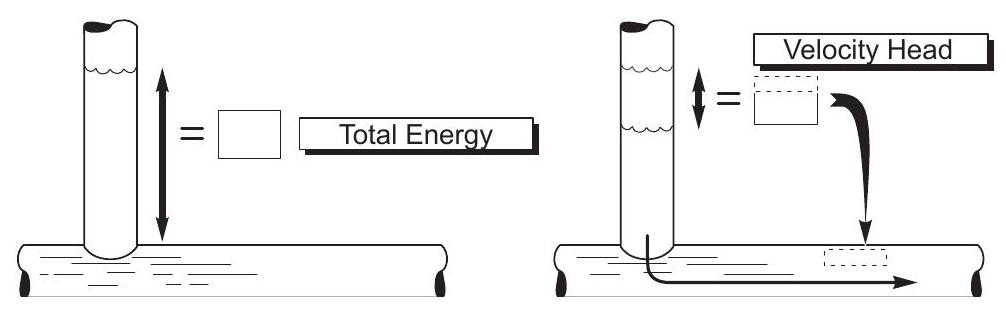
\includegraphics[scale=0.25]{2022_11_03_65aa625ded296bdfd01fg-20}
\end{center}
\textbf{Total Dynamic Head: }  Total dynamic head (TDH) is a theoretical distance. It is the static head, velocity head and headloss required to get the water from one point to another.

The horsepower output of an electric motor is directly reflected to the amperage that the motor draws. Any increase in horsepower requirements will give a corresponding increase in amperage.

\textbf{Cavitation: }  Cavitation in pumps is the rapid creation and subsequent collapse of air bubbles occuring as a result of the inlet pressure falling below the design inlet pressure or when the pump is operating at a flow rate higher than the design flow rate. This collapse of the air bubbles typically manifests as a pinging or crackling noise.  Cavitation is undesirable because it can damage the impeller, cause noise and vibration, and decrease pump efficiency.

\begin{figure}[h]
\begin{center}
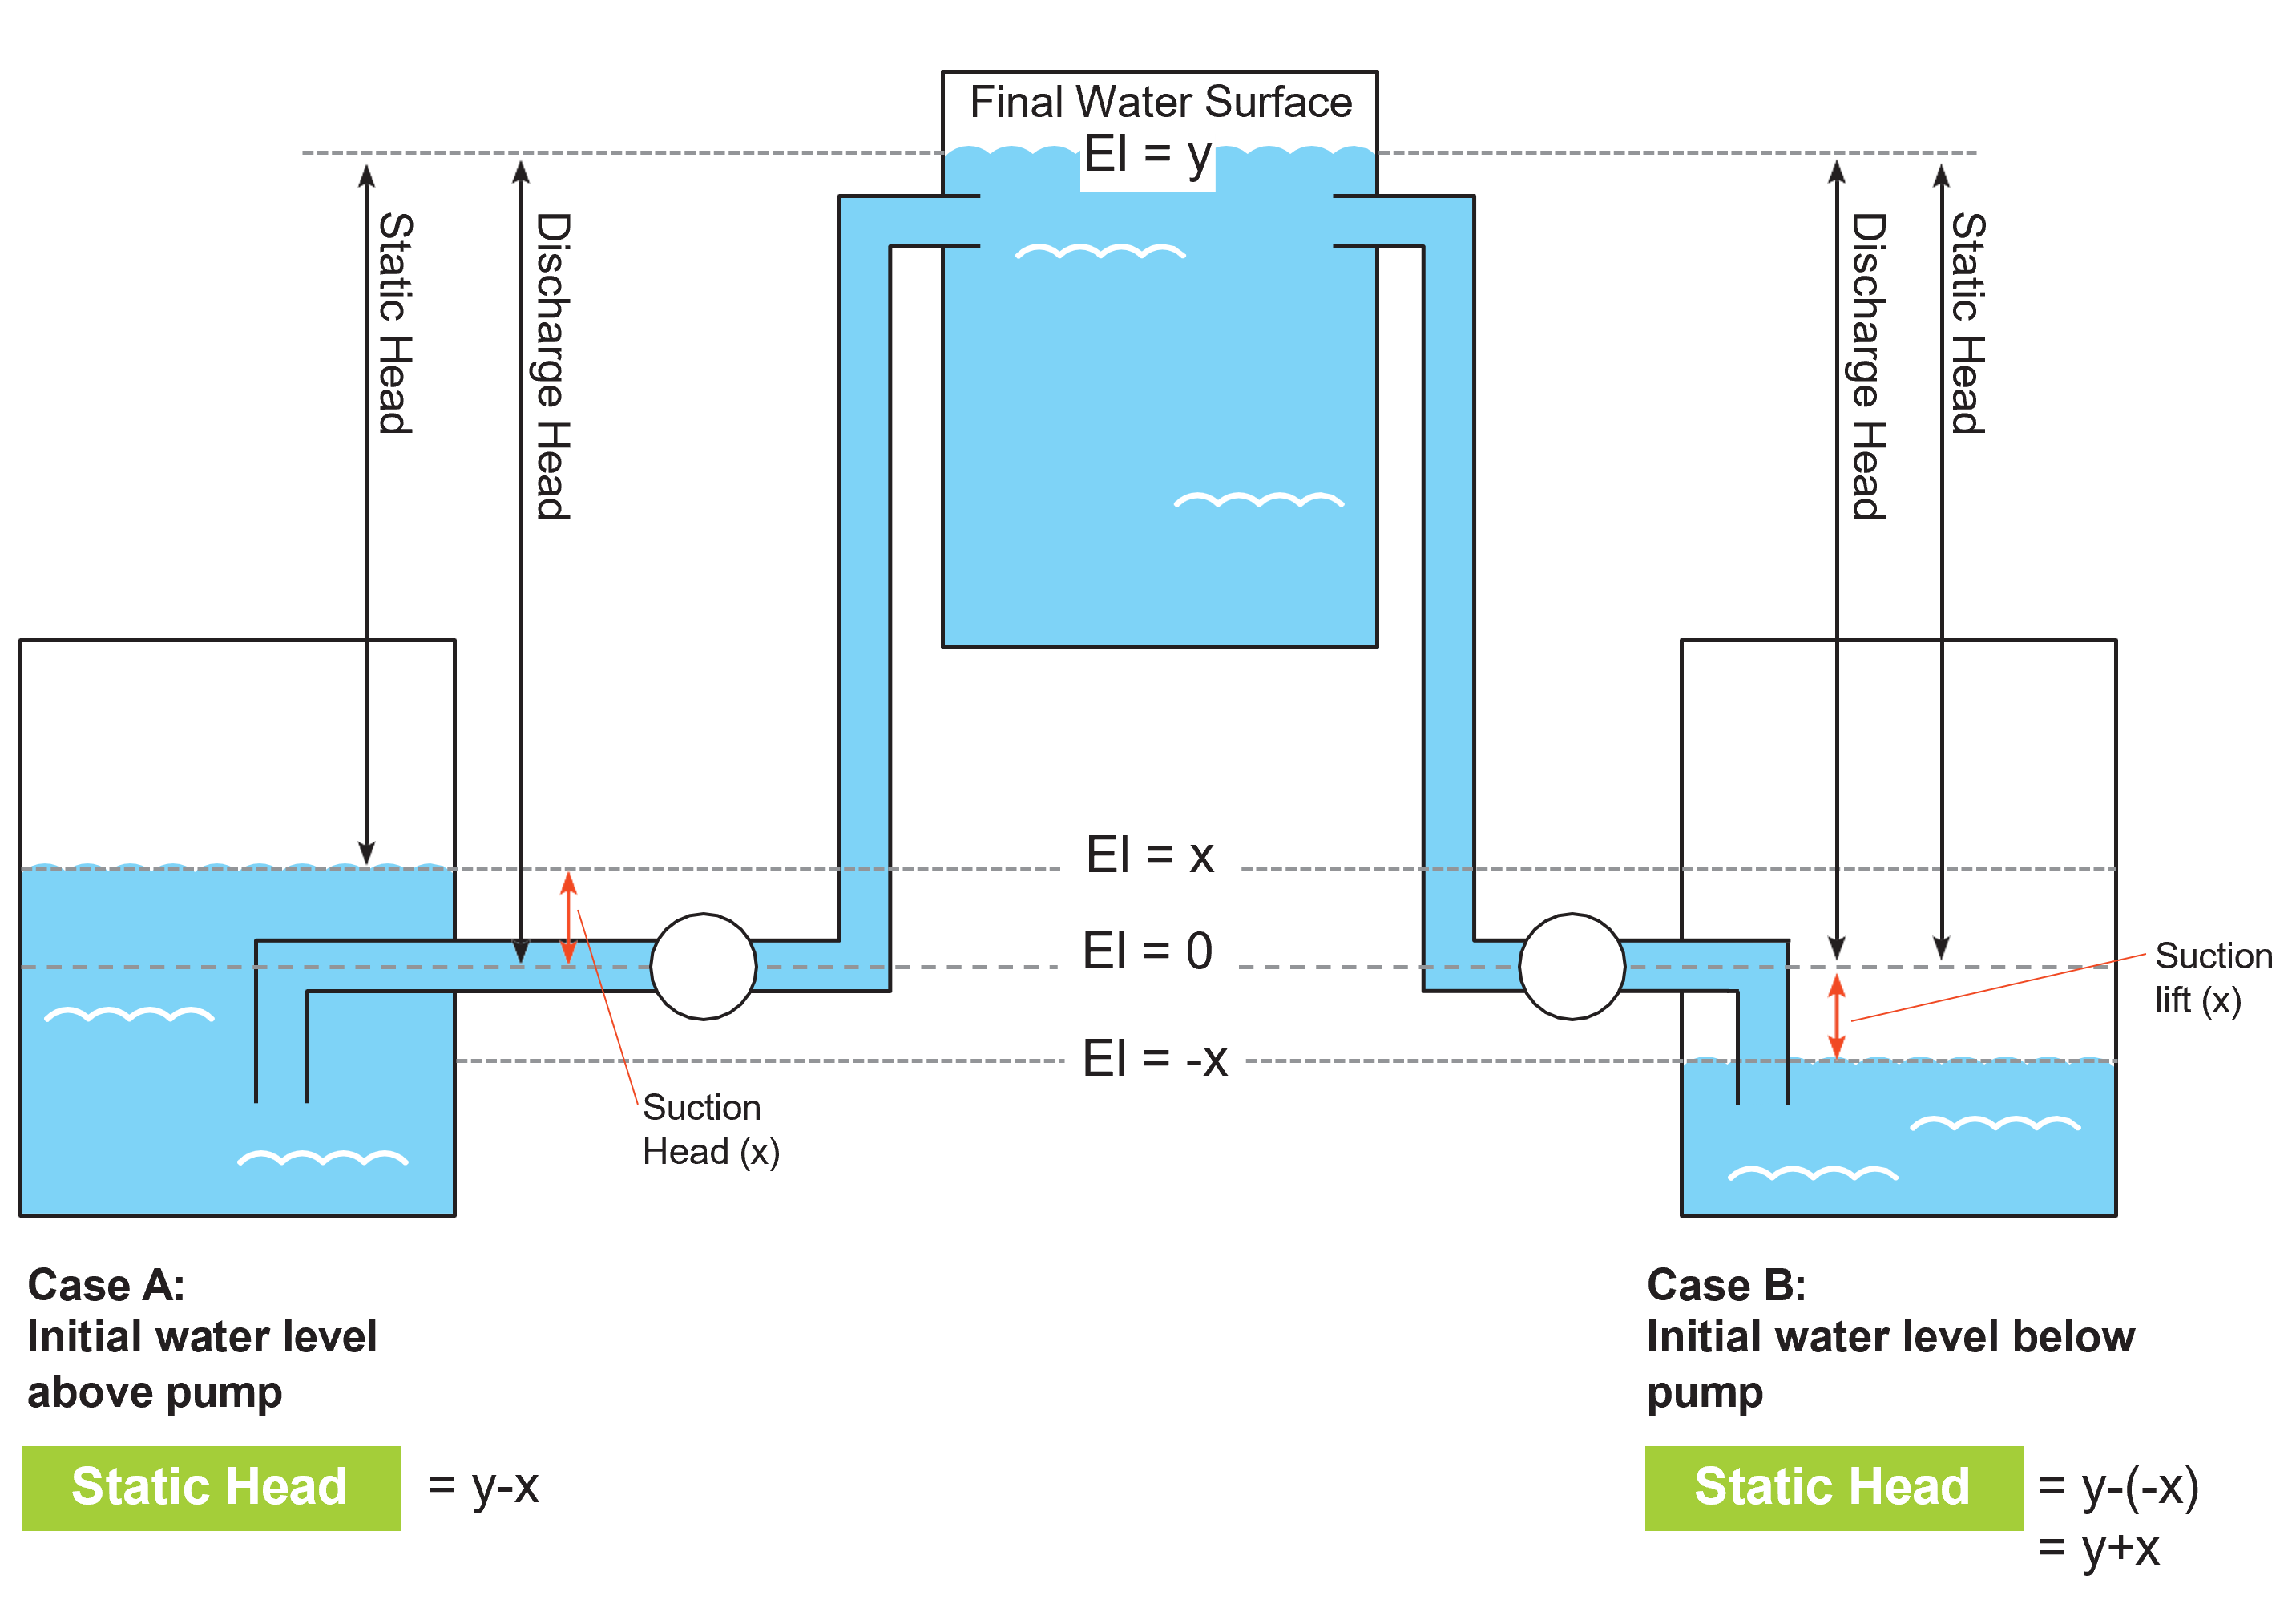
\includegraphics[scale=0.6]{CalculatingStaticHead}\\
\includegraphics[scale=0.6]{PumpHead}\\
\end{center}
\end{figure}

\newpage
\subsection{Pumping Rate Calculations}\index{Pumping Rate Calculations}
\begin{itemize}
\item \texthl{For calculating volume pumped given the pump flow rate:} Multiply the pump flow rate by the time interval\\
\textbf{Make sure:}
\begin{itemize}
\item The time units - in the given time interval and in the pump flow rate match
\end{itemize}
\item \texthl{For calculating time to pump a certain volume:}
\begin{enumerate}[Step 1.]
\item Calculate the total volume pumped
\item Divide the total volume by the pump flow rate
\end{enumerate}
\textbf{Make sure:}
\begin{itemize}
\item The volume units - in the volume that needs to be pumped and in the pump flow rate match
\item The time unit in the pump flow rate needs to be converted to the time unit that you need the answer in
\end{itemize}
\end{itemize}
% \end{enumerate}

\textbf{Example 1:}  A pump is set to pump 5 minutes each hour. It pumps at the rate of 35 gpm. How many gallons of water are pumped each day?\\
Solution:\\
$\dfrac{35 \enspace gal \enspace sludge}{\cancel{min}}*\dfrac{5 \enspace \cancel{min}}{\cancel{hr}} *\dfrac{24 \enspace \cancel{hr}}{day}=\boxed{\dfrac{4,200 \enspace gallons}{day}}$\\
\vspace{0.5cm}

\textbf{Example 2:}  A pump operates 5 minutes each 15 minute interval.  If the pump capacity is 60 gpm, how many gallons are pumped daily?

$\dfrac{60 \enspace gal \enspace sludge}{\xcancel{min}}*\dfrac{5 \enspace \xcancel{min}}{15 \enspace \cancel{min}}*1440\dfrac{\cancel{min}}{day}=\boxed{\dfrac {28,800 \enspace gal \enspace sludge }{day}}$\\
\vspace{0.5cm}

\textbf{Example 3:}  Given the tank is 10ft wide, 12 ft long and 18 ft deep tank including 2 ft of freeboard when filled to capacity. How much time (minutes) will be required to pump down this tank to a depth of 2 ft when the tank is at maximum capacity using a 600 GPM pump\\
Solution:\\
\vspace{0.5cm}


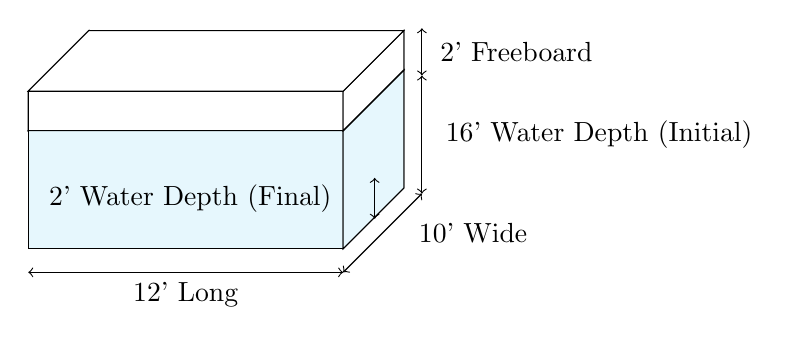
\begin{tikzpicture}

\pgfmathsetmacro{\cubexx}{4}
\pgfmathsetmacro{\cubeyy}{1.5}
\pgfmathsetmacro{\cubezz}{2}
\pgfmathsetmacro{\cubex}{4}
\pgfmathsetmacro{\cubey}{0.5}
\pgfmathsetmacro{\cubez}{2}
\pgfmathsetmacro{\cubexxx}{4}
\pgfmathsetmacro{\cubeyyy}{4}
\filldraw [fill=cyan!10!white, draw=black] (0,-\cubey,0) -- ++(-\cubexx,0,0) -- ++(0,-\cubeyy,0) -- ++(\cubexx,0,0) -- cycle ;
\filldraw [fill=cyan!0!white, draw=black] (0,-\cubey,0) -- ++(0,0,-\cubezz) -- ++(0,-\cubeyy,0) -- ++(0,0,\cubezz) -- cycle;
\filldraw [fill=cyan!10!white, draw=black] (0,-\cubey,0) -- ++(0,0,-\cubezz) -- ++(0,-\cubeyy,0) -- ++(0,0,\cubezz) -- cycle;
%\filldraw [fill=cyan!10!white, draw=black] (0,-\cubey,0) -- ++(-\cubexx,0,0) -- ++(0,0,-\cubezz) -- ++(\cubexx,0,0) -- cycle;
%%%\draw (0,-0.5,0) -- ++(-\cubex,0,0) -- ++(0,-\cubey,-\cubez) -- ++(\cubex,0,0) -- cycle;
\draw (-\cubex,0,0) -- ++(0,0,-\cubez) -- ++(0,-\cubey,0) -- ++(0,0,\cubez) -- cycle;
\draw (0,-\cubey,0) -- ++(-\cubex,0,0) -- ++(0,0,-\cubez) -- ++(\cubex,0,0) -- cycle;
\filldraw [fill=white, draw=black] (0,0,0) -- ++(-\cubex,0,0) -- ++(0,-\cubey,0) -- ++(\cubex,0,0) -- cycle ;
\filldraw [fill=white, draw=black] (0,0,0) -- ++(0,0,-\cubez) -- ++(0,-\cubey,0) -- ++(0,0,\cubez) -- cycle;
\filldraw [fill=white, draw=black] (0,0,0) -- ++(0,0,-\cubez) -- ++(0,-\cubey,0) -- ++(0,0,\cubez) -- cycle;
\filldraw [fill=white, draw=black] (0,0,0) -- ++(-\cubex,0,0) -- ++(0,0,-\cubez) -- ++(\cubex,0,0) -- cycle;

%\filldraw [fill=RoyalBlue!10!white, draw=black] (0,-1.5,0) -- ++(-\cubex,0,0) -- ++(0,-\cubey,0) -- ++(\cubex,0,0) -- cycle ;

%\filldraw [fill=RoyalBlue!10!white, draw=black] (0,-1.5,0) -- ++(0,0,-\cubez) -- ++(0,-\cubey,0) -- ++(0,0,\cubez) -- cycle;



%%\draw (0,-0.5,0) -- ++(-\cubex,0,0) -- ++(0,0,-\cubez) -- ++(\cubex,0,0) -- cycle;
%%\filldraw [fill=white, draw=black] (-\cubex,0,0) -- ++(0,0,-\cubez) -- ++(0,-\cubey,0) -- ++(0,0,\cubez) -- cycle;
%%\filldraw [fill=white, draw=black] (0,-\cubey,0) -- ++(-\cubex,0,0) -- ++(0,0,-\cubez) -- ++(\cubex,0,0) -- cycle ;

\draw [<->] (-4,-2.3) -- (0,-2.3) node [midway, below] {12' Long};
\draw [<->] (1,-1.3) -- (1,.2) node [midway, midway] {\hspace{4.5cm}16' Water Depth (Initial)};
\draw [<->] (0.4,-1.62) -- (0.4,-1.1) node [midway, midway] {\hspace{-4.8cm} 2' Water Depth (Final)};
\draw [<->] (1,.8) -- (1,.2) node [midway, midway] {\hspace{2.4cm}2' Freeboard};
\draw [<->] (1,-1.3) -- (0,-2.3) node [midway, midway] {\hspace{2.3cm}10' Wide};
\end{tikzpicture}\\
Volume to be pumped=$12 \enspace ft*10 \enspace ft *(16-2)\enspace ft=1,680ft^3$\\
\vspace{0.3cm}
$\implies \dfrac{1,680\cancel{ft^3}*7.48\dfrac{\cancel{gal}}{\cancel{ft^3}}}{600\dfrac{\cancel{gal}}{min}}=\boxed{21min}$

% \begin{tcolorbox}[breakable, enhanced,
% colframe=blue!25,
% colback=blue!10,
% coltitle=blue!20!black,  
% title= Practice Problems]
% \begin{enumerate}
% \item Convert 45 psi to feet of head

% \item How long (in minutes) will it take to pump down 25 feet of water in a 110 ft diameter cylindrical tank when using a 1420 gpm pump\\

% \item How long will it take (hrs) to fill a 2 ac-ft pond if the pumping rate is 400 GPM?

% \item A tank is filling at the rate of 300 gpm for a 20 minute period. How many of water will be contained in the tank at the end of 16 minutes?
% \end{enumerate}
% \end{tcolorbox}






\subsection{Power Requirements for Pumping}\index{Power Requirements for Pumping}
\begin{center}
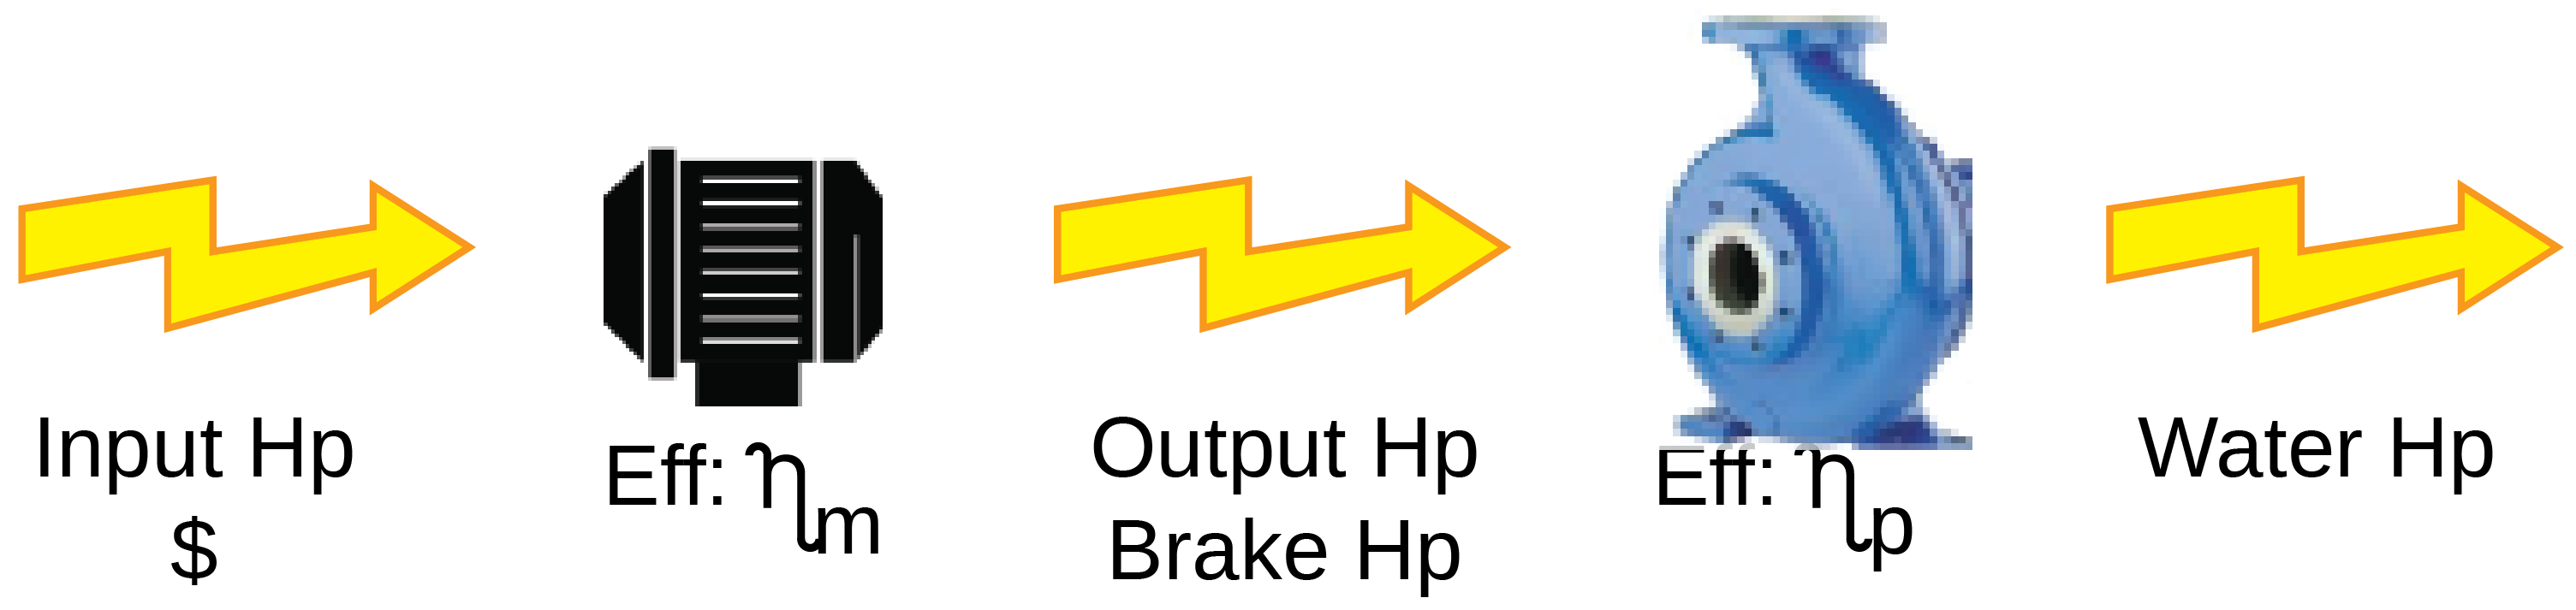
\includegraphics[scale=0.12]{PumpProblem}\\
\end{center}
Where:\\
\begin{itemize}
\item \textbf{Input Hp} is the input power to the motor which produces the \textbf{Output Hp or Brake Hp} - the mechanical power which runs the pump.  
\item The ratio of Output Hp and Input Hp is the motor efficiency - $\eta_m$.
\item The Output Hp is the input power (Brake Hp) to the pump to pump the water.
\item Water Hp is the rate of energy transferred to the water being pumped and can be calculated by the formula:\\
$$\dfrac{\mathrm{H \enspace - \enspace Head \enspace of \enspace water \enspace (ft) \enspace * \enspace Q \enspace - \enspace Flow \enspace (GPM)}}{3,960 \enspace \mathrm{(Conversion \enspace factor \enspace for \enspace converting \enspace GPM-ft \enspace to \enspace Hp)}}$$
\item The ratio of Output Hp and Water Hp is the pump efficiency - $\eta_p$.
\end{itemize}
\subsection{Example Problems}
\begin{enumerate}


\item 1 MGD is pumped against a 14’ head.  What is the water Hp?  The pump mechanical efficiency is 85\%.  What is the brake horsepower?\\
\vspace{0.4cm}
water Hp = flow * head\\
\vspace{0.4cm}
$\dfrac{1,000,000 \enspace gal}{day}*\dfrac{day}{1440 \enspace min}*14 \enspace ft*\dfrac{Hp}{3,960 \enspace GPM-ft}=\boxed{Water \enspace Hp = 2.46 \enspace Hp}$\\
\vspace{0.4cm}
pump Hp = brake Hp * pump efficiency\\
\vspace{0.4cm}
$Brake \enspace Hp = \dfrac{2.46}{0.85}=\boxed{Brake \enspace Hp=2.89Hp}$\\
\vspace{0.4cm}

\item A flow of 200 gpm  is pumped against a total head of 4.0 feet. The pump is 78\% efficient and the motor' is 90\% efficient. Calculate the input Hp.\\
\vspace{0.4cm}
water Hp = flow * head\\
\vspace{0.2cm}
$200GPM*4ft*\dfrac{Hp}{3,960 GPM-ft}=0.2Hp$\\
\vspace{0.4cm}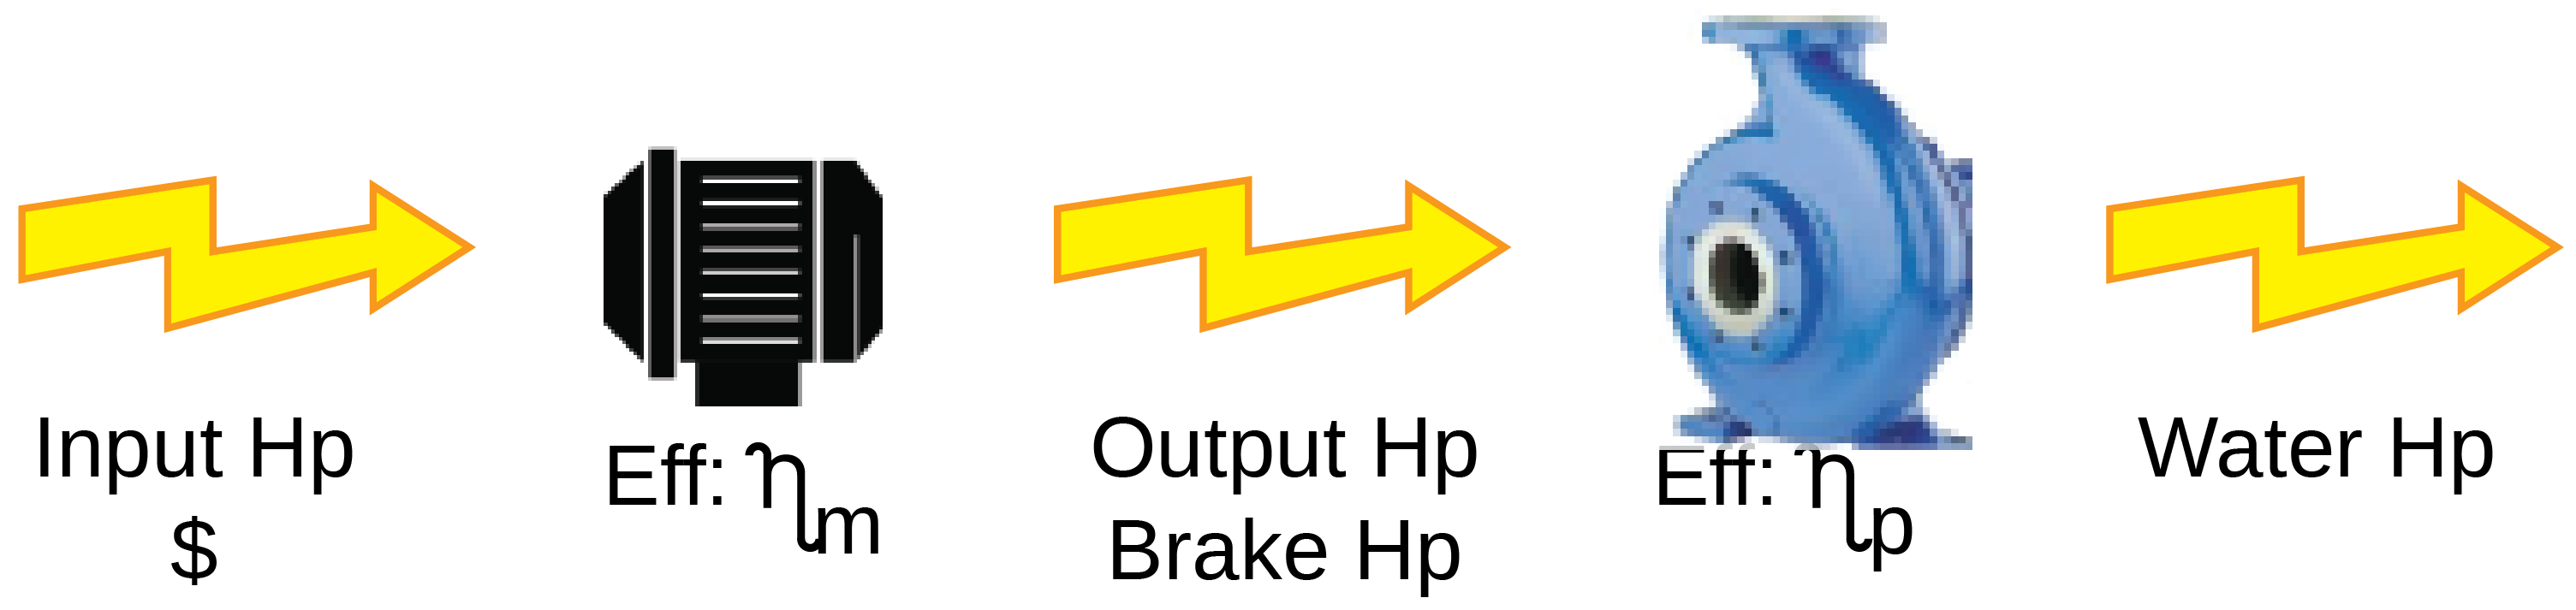
\includegraphics[scale=0.08]{PumpProblem}\\
water Hp=brake Hp*pump efficiency, and\\
brake Hp=input Hp*motor efficiency\\
Therefore, water Hp=input Hp*motor efficiency*pump efficiency\\
\vspace{0.4cm}
input Hp=$\dfrac{water \enspace Hp}{motor \enspace efficiency*pump \enspace efficiency}=\dfrac{0.2}{0.9*0.78}=\boxed{0.28Hp}$
\vspace{0.2cm}0
\end{enumerate}

% \begin{tcolorbox}[breakable, enhanced,
% colframe=blue!25,
% colback=blue!10,
% coltitle=blue!20!black,  
% title= Practice Problems]
% \begin{enumerate}

%   \item If a pump is operating at 2,200 gpm and 60 feet of head, what is the water
% horsepower? If the pump efficiency is 71\%, what is the brake horsepower?

% \item The water horsepower of a pump is $10 \mathrm{Hp}$ and the brake horsepower output of the motor is $15.4 \mathrm{Hp}$. What is the efficiency of the pump?

% \item The water horsepower of a pump is $25 \mathrm{Hp}$ and the brake horsepower output of the motor is $48 \mathrm{Hp}$. What is the efficiency of the pump?

% \item The efficiency of a well pump is determined to be $75 \%$. The efficiency of the motor is estimated at $94 \%$. What is the efficiency of the well?

% \item If a motor is $85 \%$ efficient and the output of the motor is determined to be 10
% $\mathrm{BHp}$, what is the electrical horsepower requirement of the motor?

% \item The water horsepower of a well with a submersible pump has been calculated at 8.2 WHp. The Output of the electric motor is measured as $10.3 \mathrm{BHp}$. What is the efficiency of the pump?

%   \item Water is being pumped from a reservoir to a storage tank on a hill. The elevation difference between water levels is 1200 feet. Find the pump size (in Hp) required to fill the tank at a rate of 120 gpm.
  
%   \end{enumerate}
%   \end{tcolorbox}